\chapter{Methodology, consideration and decision on alternative solutions}

Looking at the "State of the art" chapter, I want to develop a solution that incorporates as many of the strengths of existing solutions as possible. Considering the available resources, the most effective solution is a \textbf{software-based solution} that interacts with the sound card, display, mouse, and keyboard available in a standard computer.

This approach enables me to implement a solution that takes into account the followings strength points:

\begin{itemize}
	\item \textbf{Analysis capabilities:} This must include: spectrogram, 31-band graphic display, delay measurement, phase measurement, RT60 measurement, and waterfall diagram.
	
	\item \textbf{Processing capabilities:} It must be able to process a live signal using an equalizer implemented with digital filters.
	
	\item \textbf{Signal management:} It must handle an external clean signal, a signal that has passed through the system, and output a processed signal.
	
	\item \textbf{Real time:} The system must operate in live situations, meaning it must be capable of analyzing and processing audio in real time.
	
	\item \textbf{Low resource usage:} The solution should be usable by anyone with a PC, a sound card, a microphone, and a speaker—without requiring any other high-end hardware.
\end{itemize}

Of course, the type and quality of the sound card and microphone will be critical to obtaining accurate and realistic results. Under optimal conditions, a high-resolution sound card with good SNR, along with a high-quality measurement microphone, is required. These microphones are typically small-diaphragm, condenser, omnidirectional, with a flat frequency response and good signal-to-noise ratio.

The importance of the speaker depends on whether we consider it part of the system (a fixed speaker that is part of the room) or simply a tool used to excite the room. In the first case, the program should correct the speaker's imperfections, as it is part of the system being analyzed and corrected. The only requirement for this speaker is that it must be able to reproduce the full frequency spectrum that will be analyzed and corrected.

However, in the second case, it is very important for the speaker to have the flattest response possible, since any imperfections in the speaker will introduce false data about the room acoustics.

I will be using a Behringer U-Phoria UMC204HD sound card, an old Electro-Voice desktop microphone, and an old AIWA SX-NAVH1000 home hi-fi speaker. These are not the best hardware for analysis tools, but they are sufficient to develop the software under home conditions.

\begin{figure}[H]
	\centering
	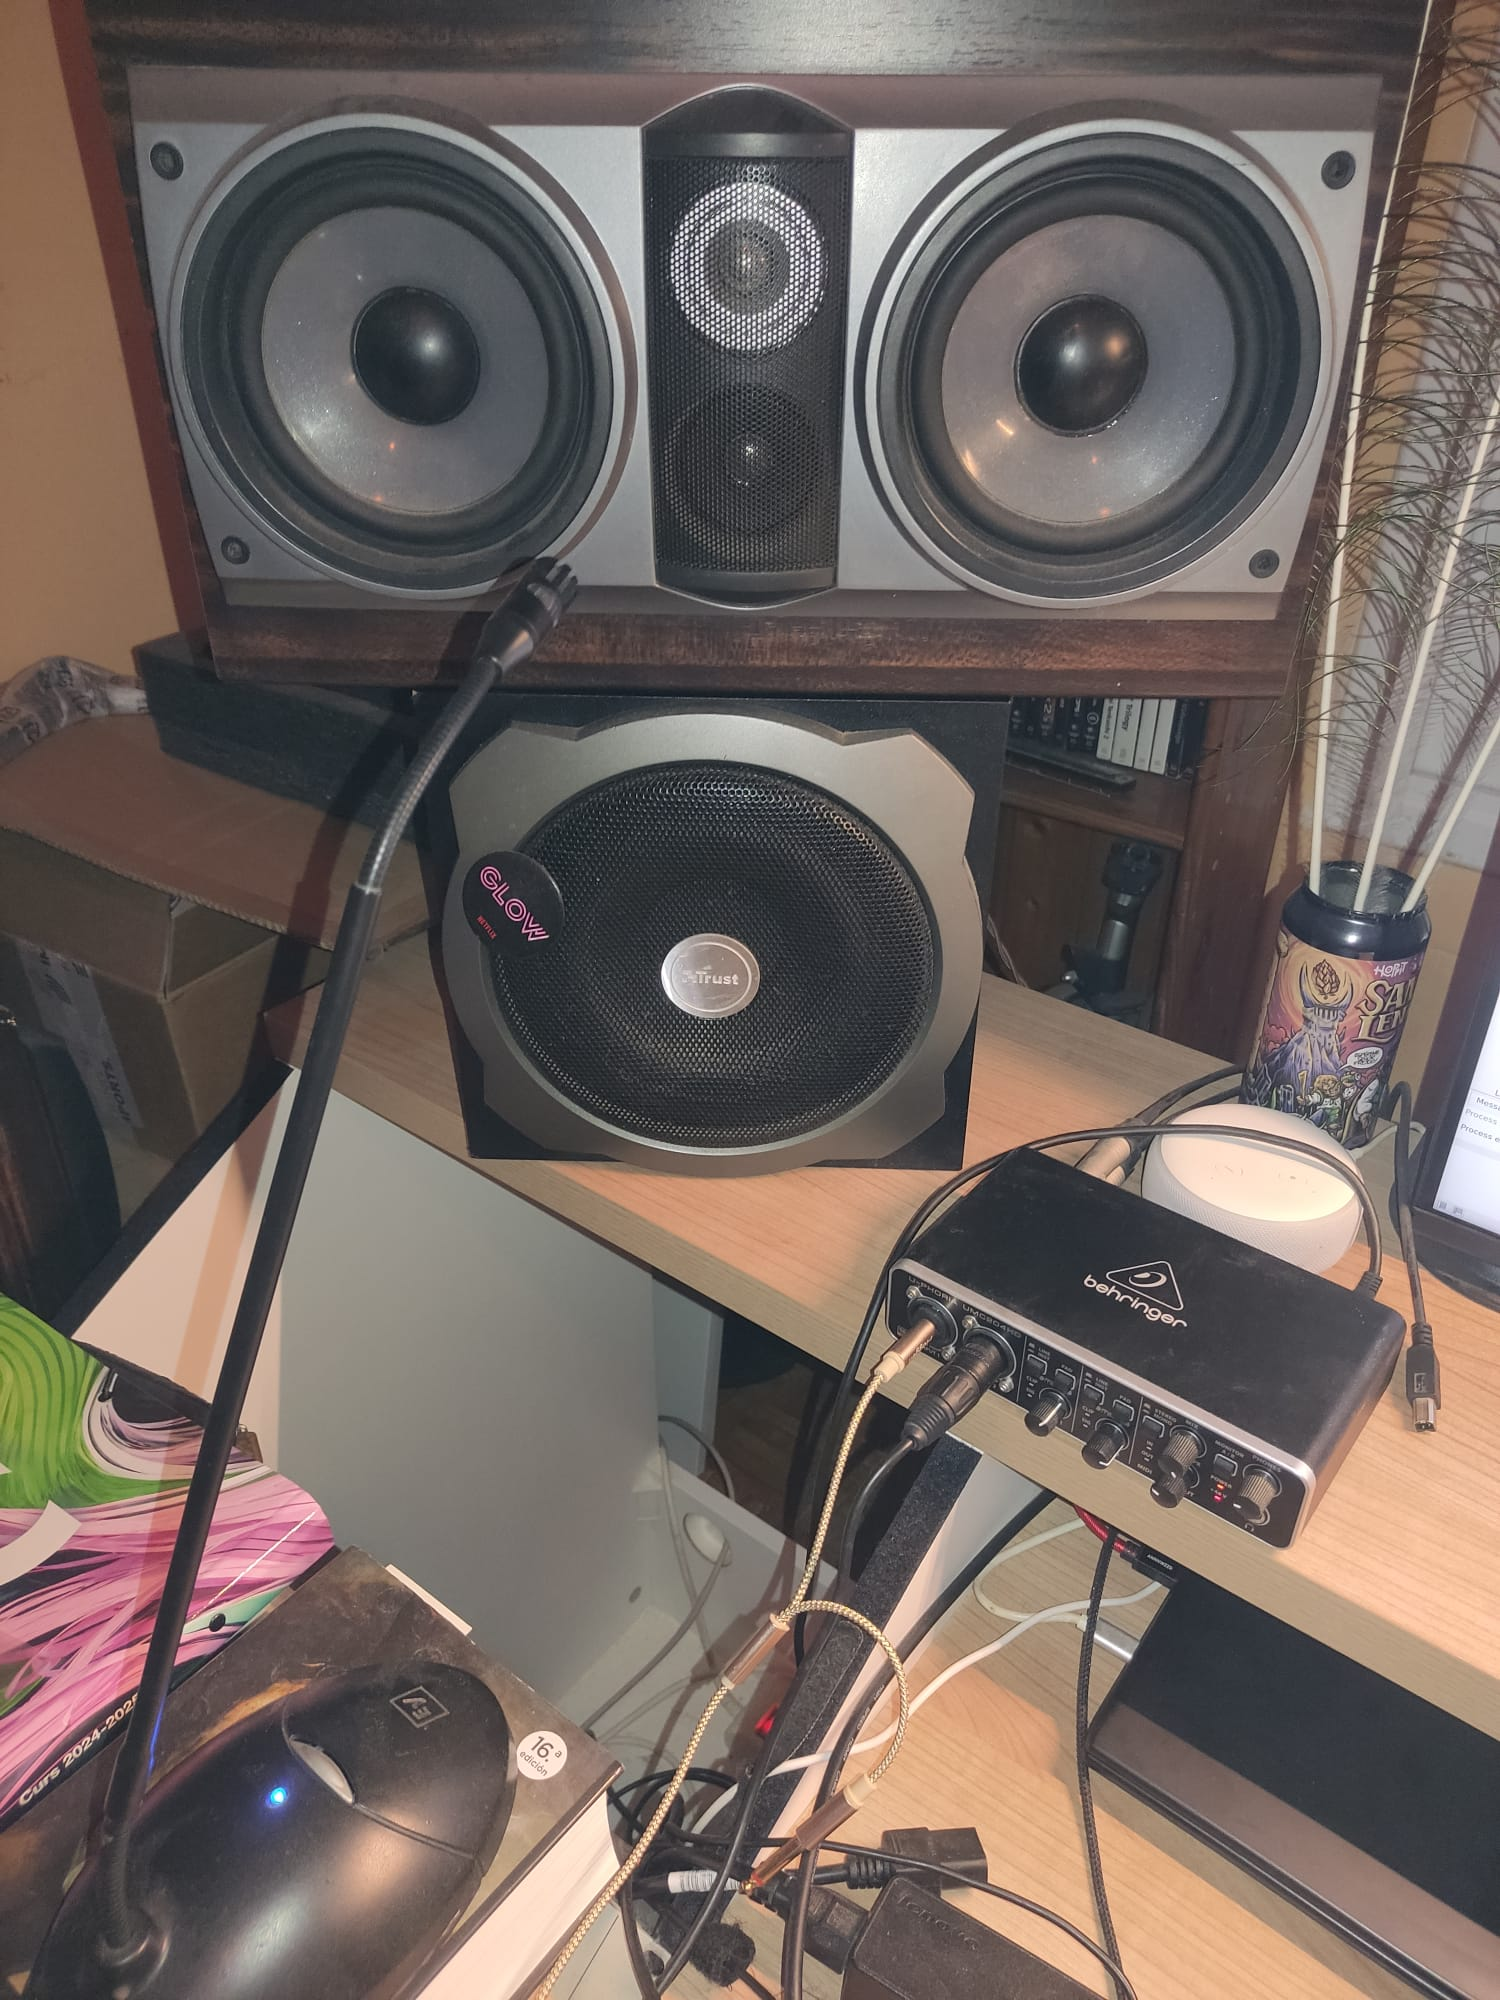
\includegraphics[width=0.6
	\linewidth]{Figures/HomeSetUp.jpeg}
	\caption[Home setup]{Home setup showing the sound card, the speaker, and the microphone.}
	\label{fig:Home Setup}
\end{figure}

As a computer, I will be using a laptop running Ubuntu 22.04.5 LTS and Python 3.

In order to achieve the overall goal, the program to be developed needs a set of tools that must communicate with each other. To achieve this, a \textbf{GUI} (\textit{Graphical User Interface}) will be very helpful, and it should be easy and intuitive to use.



